% DO NOT COMPILE THIS FILE DIRECTLY!
% This is included by the other .tex files.

\begin{frame}[t,plain]
\titlepage
\end{frame}

\begin{frame}
    \frametitle{Objectives}
    \begin{itemize}
        \item Identify non-technical data that can be useful for an investigation,
        \item Illustrate how non-technical and technical data can interact to produce meaninful insights,
        \item Model these interactions,
        \item Outline what Socio-Technical intercations are useful to share.
    \end{itemize}

    \note[item]{A note for the slide handout}
\end{frame}


\begin{frame}
	\frametitle{We live in Socio-Technical Systems}

    Computer and their security is linked to human activities:

    \begin{itemize}
        \item Technical traces show human activities,
        \item Technical traces can convey human intent,
        \item Human interactions can explain and give context to Technical traces,
        \item CyberCrime requires infrastructures and logistics that are discussed between humans,
	\item TTPS are discussed and exchanged,
	\item Human interaction can help attributing an attack,
	\item Human interaction can help deciphering intent and motives, and discriminate human error from sabotage.
    \end{itemize}

    \note[item]{A note for the slide handout}
\end{frame}


\begin{frame}
	\frametitle{Plan}
    \begin{itemize}
        \item Modeling a specific ransomware case,
        \item Using OSINT and data leaks to bring context to other ransomware cases.
    \end{itemize}

    \note[item]{A note for the slide handout}
\end{frame}

\section{Conti analysis}


\begin{frame}[fragile]
    	\frametitle{Ransomware Jabber chats leak}
	Published on Twitter:
	\begin{figure}[t]
		
\includegraphics[width=.8\textwidth]{contileaks-twitter.png}
		\centering
	\end{figure}

	Contained XMPP server logs:
	\begin{figure}[t]
		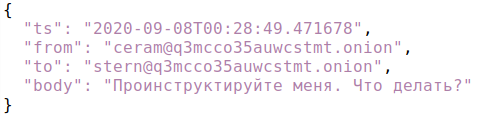
\includegraphics[width=.6\textwidth]{contileaks-json.png}
		\centering
	\end{figure}


\end{frame}


\begin{frame}[fragile]
    	\frametitle{Ransomware Jabber chats leak}
	Our goal is:

    \begin{itemize}
       	\item Dig into these Jabber chats in search for IoC and operational information
	    \item use MISP to correlate this information from past cases,
	    \item ease attribution of these past cases through IoC,
	    \item add context to past cases from the chats logs in order to ease their investigation,
	    \item support colleagues and other CSIRTs with real Intelligence.
    \end{itemize}

\end{frame}

\begin{frame}
    \frametitle{Ransomware Jabber chats leak}
	We use AIL\footnote{\url{https://ail-project.org/}} to dig into the data:
    \begin{itemize}
        \item AIL processes the data and search for relevant information
    	\begin{itemize}
		\item PGP keys,
		\item Bitcoin addresses, maybe others,
		\item onion hidden services.
    	\end{itemize}
	\item Once we find relevant information we push it into MISP,
	\item we use MISP correlation engine to find relevant past cases.
    \end{itemize}
	TODO: checking if the data we have actually allows that
    \note[item]{A note for the slide handout}
\end{frame}



\begin{frame}
    \frametitle{Ransomware Jabber chats leak}
    \begin{itemize}
        \item A bullet point
    \end{itemize}

    \note[item]{A note for the slide handout}
\end{frame}



\begin{frame}
    \frametitle{Ransomware Jabber chats leak}
    \begin{itemize}
        \item A bullet point
    \end{itemize}

    \note[item]{A note for the slide handout}
\end{frame}



\begin{frame}
    \frametitle{Slide title}
    \begin{itemize}
        \item A bullet point
    \end{itemize}

    \note[item]{A note for the slide handout}
\end{frame}



\begin{frame}
    \frametitle{Slide title}
    \begin{itemize}
        \item A bullet point
    \end{itemize}

    \note[item]{A note for the slide handout}
\end{frame}



\begin{frame}
    \frametitle{Slide title}
    \begin{itemize}
        \item A bullet point
    \end{itemize}

    \note[item]{A note for the slide handout}
\end{frame}



\begin{frame}
    \frametitle{Slide title}
    \begin{itemize}
        \item A bullet point
    \end{itemize}

    \note[item]{A note for the slide handout}
\end{frame}

